% !TeX root = ../main.tex

\chapter{系统需求分析}

本章主要介绍数据湖分析系统的需求分析过程,主要包括系统概述、功能性
需求分析、非功性需求分析三部分。针对公司目前面临的挑战和业务痛点,梳理业
务流程,确定项目需求。然后将需求划分为不同的模块,确定不同模块包含的功能
点,进行用例图展示,为后续的系统设计以及开发测试工作奠定基础。

\section{系统概述}

虽然数据湖在企业内部的需求很高,但客户使用的门槛较高,需要根据Apache Iceberg
官网的教程编写java程序来实现数据的入湖或者读取,这就对不太熟悉java的客户来说
不太友好,并且Iceberg后续的运维成本对于客户来说也比较高。因此,我们开发了数据
湖分析系统,数据湖分析系统可以轻松完成T+0实时入湖,支持批流融合、秒级分析、事务语义、挖掘和探索数据价值等。

DLA底层基于Apache Iceberg作为数据湖载体,开发框架使用Spring Boot,包含数
据源管理、元数据管理、数据入湖、数据探索四大模块,并且我们还在Iceberg侧实现了
小文件合并优化的功能,不但减少了小文件的数量增强了Iceberg的查询能力,而且还降低了用户的运维成本。

\section{系统功能性需求}

上一小节系统概述中,将数据湖分析系统划分为四大模块,在本节中将针对每一个模块进行详细分析。

\subsection{数据源管理模块}

数据源是入湖任务的前提要求,注册相应数据源,创建入湖任务时即可根据创建的数据源选择对应的源表。
数据源管理模块主要对数据源进行管理,其中关系型数据库支持Mysql,消息队列数据源支持Tube、Kafka、
Pulsar[17]等数据源;支持数据源创建、查看、编辑、删除功能。数据源管理模块的需求用例图如图3.1所示:

\begin{figure}[h]
  \centering
  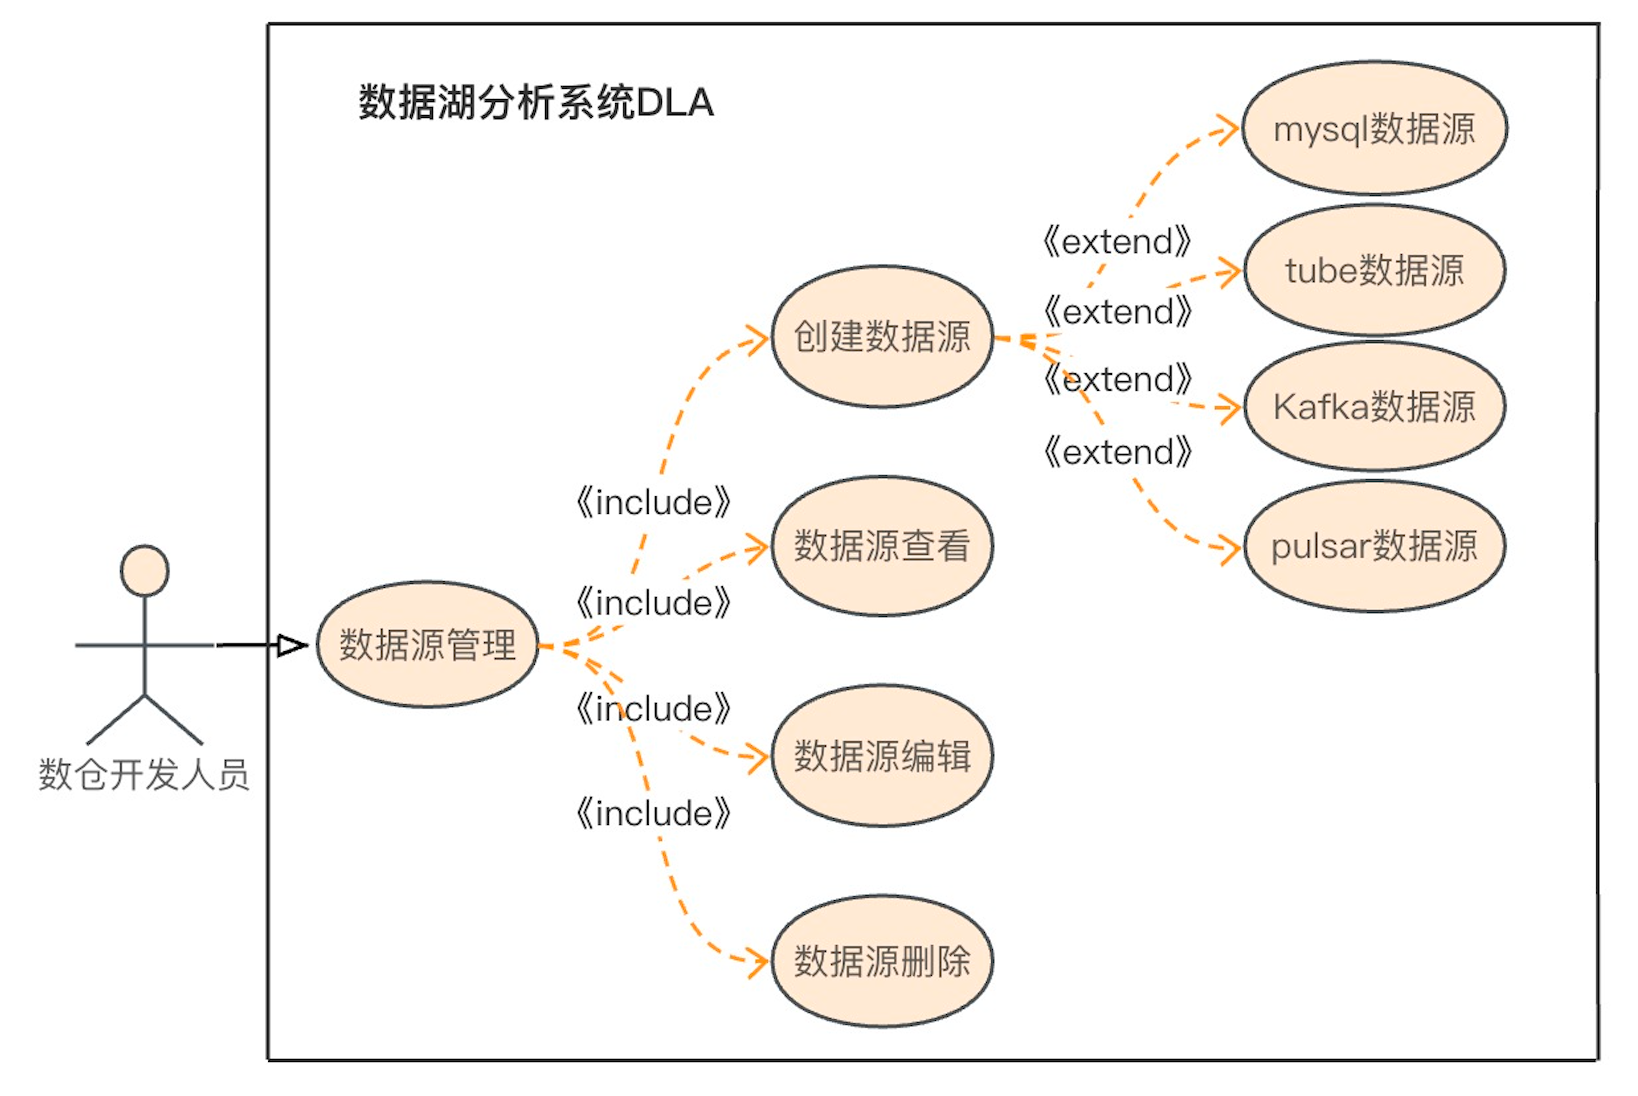
\includegraphics[width=1.0\textwidth]{数据源用例图.png}
  \caption{数据源管理模块用例图}
  \label{fig:badge}
\end{figure}

\subsection{元数据管理模块}

元数据(Metadata)是描述其它数据的数据(data about other data)[15],
或者说是用于提供某种资源的有关信息的结构数据(structured data)。元数据是
描述信息资源或数据等对象的数据,其使用目的在于:识别资源;评价资源;追踪资源
在使用过程中的变化;实现简单高效地管理大量网络化数据;实现信息资源的有效发现、查找、一体化组织和对使用资源的有效管理。

这里的元数据是描述iceberg表的,iceberg表即目标表,是入湖任务的前提要求,
可以创建新表或者关联已有的表,在创建入湖任务时即可选择对应的目标表。元数据管
理模块主要对iceberg元数据进行管理,包含四个主要的功能,分别是数据优化、表的
创建、表的编辑、表的查看。其中数据优化功能包括:合并小文件、清理过期快照数据、
删除孤儿文件、生命周期管理,而其中的小文件合并,我们在iceberg侧做了很大的优化,
会在接下来的章节进行介绍。数据优化功能的目的是降低用户的运维成本,使用户可以一
键启动该服务,不需要自己写java程序来优化,并会根据表的若干指标及历史执行情况
判断所需资源,并配有告警机制,及时通知专业运维处理;表的创建既可以在DLA上创建
新的iceberg表,也可以关联在其它平台上已创建的iceberg表;表的编辑可以将创建过
的表进行修改编辑,支持字段的增加及删除操作。元数据管理模块的需求用例图如图3.2所示:

\begin{figure}[h]
  \centering
  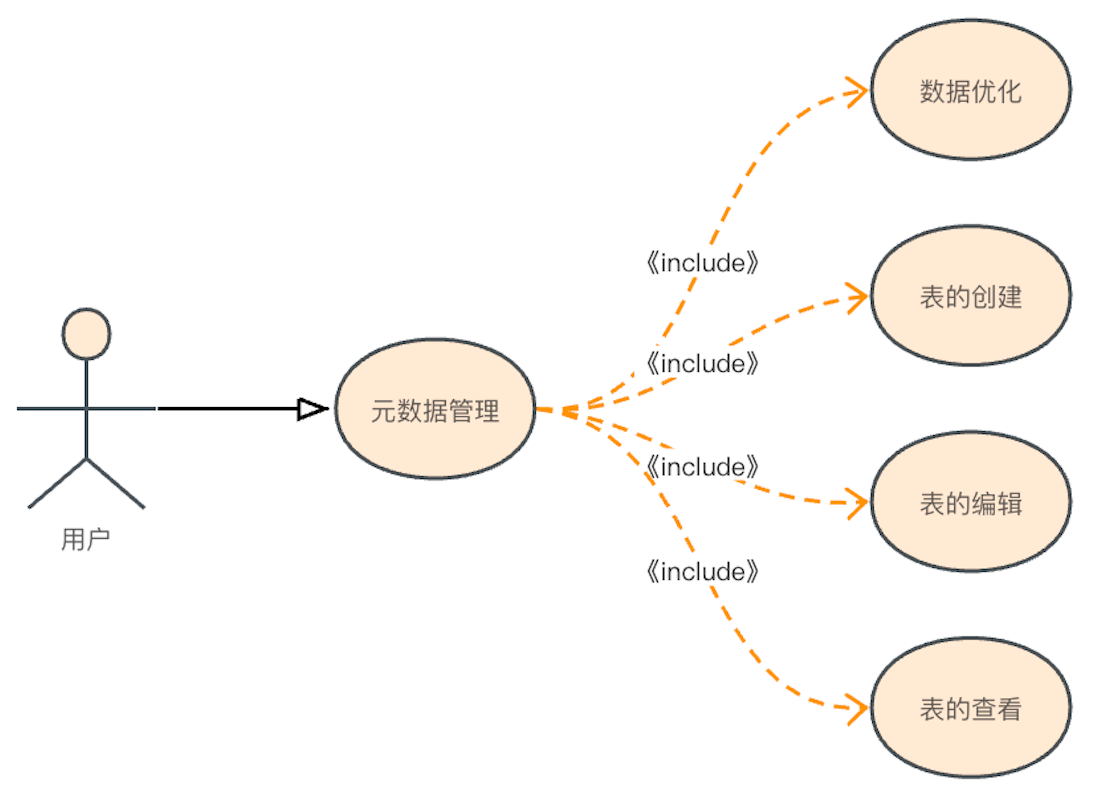
\includegraphics[width=1.0\textwidth]{元数据用例图.png}
  \caption{元数据管理模块用例图}
  \label{fig:badge}
\end{figure}

\subsection{数据入湖模块}

数据入湖功能模块是DLA系统核心流程功能,目的是用户通过该功能将源数据表流程化入湖和查看
已申请入湖任务执行情况,目前支持的入湖类型为实时入湖(tube入湖、kafka入湖、pulsar入湖)
、存量入湖(data warehouse数据入湖)、关系型数据库入湖(mysql全量入湖、mysql增量入湖)。
其中实时入湖就是流形式的入湖,底层使用的flink来实现的;存量入湖就是批形式的入湖,底层使用的
spark来实现的;关系型数据入湖是指数据源是mysql,有全量、增量两种方式,全量就是只执行一次,
增量就是需要设置时间间隔、起始时间来定时更新。数据入湖模块的需求用例图如图3.3所示:

\begin{figure}[h]
  \centering
  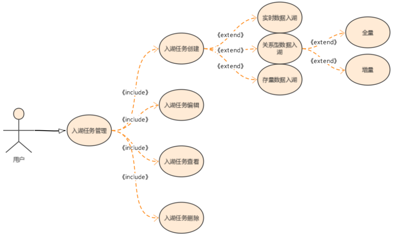
\includegraphics[width=1.0\textwidth]{数据入湖用例图.png}
  \caption{数据入湖模块用例图}
  \label{fig:badge}
\end{figure}

创建入湖任务总共需要五步:

(1)填写基础信息,根据入湖需要选择对应的入湖分类,填写必要的任务名;

(2)填写源表,实时入湖与关系型数据库入湖需要提前注册数据源,选择对应数据源表;

(3)填写目标表,所有入湖任务基本一致,支持推荐Schema功能,无需提前新建表,若目标表未创建,则任务创建时会自动的创建与源表对应的目标表,简化了创建目标表流程;

(4)查看映射预览,对源表及目标表schema映射展示,schema不一致无法进行下一步;

(5)填写参数及资源,对任务的资源进行配置。

\subsection{数据探索模块}

数据探索是数据入湖后,用户可以使用Spark、Presto、Zeppelin等引擎来进行查询分析数据,以实现数据的价值。

Spark和Presto都是通过写SQL作业来完成数据的查询分析,Presto的查询能力(select能力)突出,
可以实现秒级查询,但是Presto仅支持查询,其它的语句都不支持,相对的Spark的查询能力一般,
但是Spark支持的语句比较多,创建表、删除表、更新表、数据写入、数据删除、更新分区、表维护等
语句都是支持的。用户可以结合实际的情况灵活使用。

Zeppelin是一个基于Web的notebook,提供交互数据分析和可视化。后台支持接入多种数据处理引擎,
如spark,hive等。支持多种语言: Scala(Apache Spark)、Python(Apache Spark)、
Spark SQL、 Hive、 Markdown、Shell等。开发者可以通过实现更多的解释器来为Zeppelin添加数据引擎。

\subsection{小文件合并优化模块}

由于原有的Iceberg小文件合并功能在我们的实际应用有着诸多的问题,比如合并不及时、浪费资源、
合并资源占用计算资源过多的问题。基于以上问题,我们重新设计了小文件合并模块。

\subsubsection{分区表进行重分区}

由于实时写入 Iceberg 任务为了保证实时性,会进行高频的commit操作,
而这引起的小文件数量以及元数据数目膨胀会引起查询性能的降低,
此外文件数量的膨胀也会对存储系统如HDFS的Namenode 造成较大的压力,

对于分区表而言,数据的上游写入的每个task 的输入理论上包含这个表所有
的分区的数据,举个例子,假设一张 Iceberg 表以省份作为分区,则
如图3.4所示,InputStream-0和InputStream-1的数据理论上是包含34个省份的,
此时下游的每一个 IcebergWriter 任务都会接受到34个省份的数据,由于Iceberg
的分区信息在磁盘上是一个固定的文件夹,因此一个 IcebergWriter理论上就会生成34个文件夹,
每个文件夹对应的不同省份的数据。这里就可以发现,当我们的数据量比较大的时候,
例如我们设置Flink写入Iceberg 的这个任务的并发度是100,那么理论上HDFS
上这张表的分区文件夹的数量即为 100 * 34。假如一分钟进行一次commit 操作,
每次commit 操作都只生成一份数据文件,每分钟都会有34个省份的数据写入,
则产生的文件数量为 100 * 34 * 1 = 3400 个。

\begin{figure}[h]
  \centering
  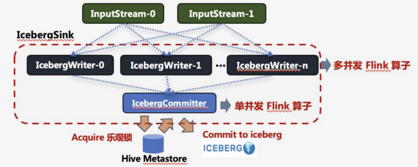
\includegraphics[width=1.0\textwidth]{重分区前的Iceberg写入示意图.png}
  \caption{重分区前的Iceberg写入示意图}
  \label{fig:badge}
\end{figure}

这里我们很容易的发现,在数据并发写入的情况下,是由于数据离散的分布在每一个task
上导致每一个task 的写操作都会包含所有的分区信息,那么很容易的想到,在inputStream
后针对分区信息将数据进行重分区,如图3.5所示,即使得每一个 IcebergWriter 之间不会有
重复的分区信息,每一个task 只会写他负责的那部分数据,这样就可以把整体的文件数量减
少并发度的量级。例如按上面的例子来说,单个 IcebergWriter 只会写 >= 1 个分
区的数据且这部分数据有且仅为这个task ,那么整体的分区文件夹数量就会减少到 34 个而非 100 * 34。

\begin{figure}[h]
  \centering
  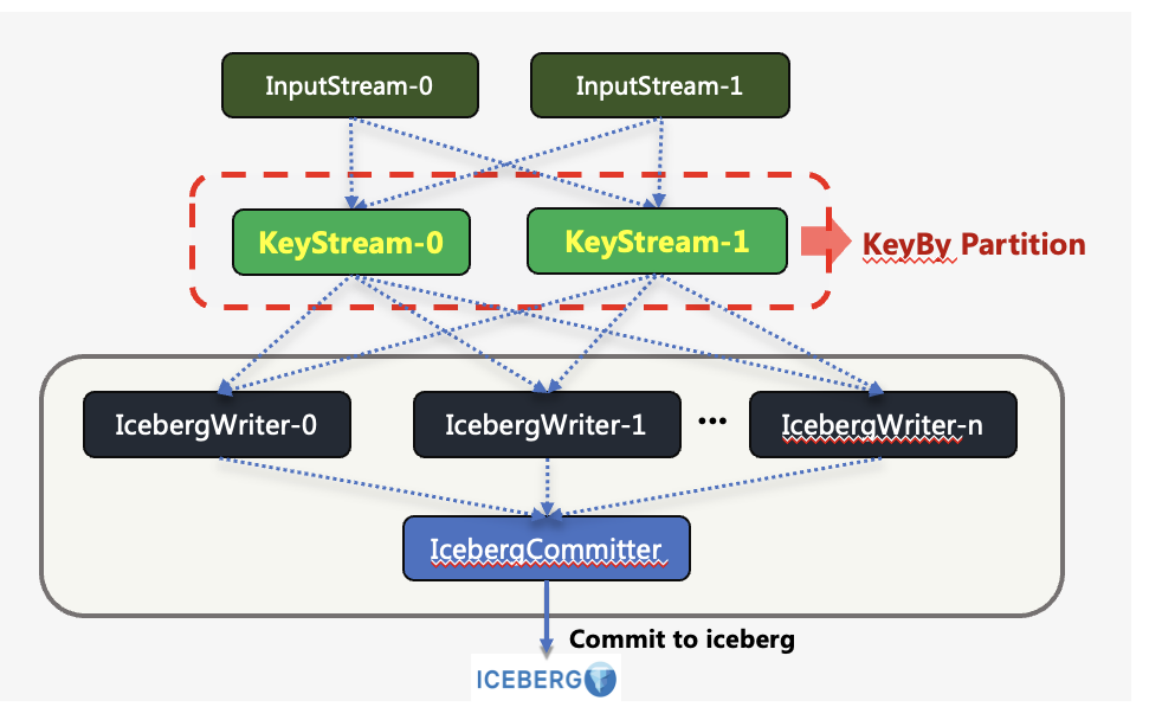
\includegraphics[width=1.0\textwidth]{进行重分区的Iceberg写入示意图.png}
  \caption{进行重分区的Iceberg写入示意图}
  \label{fig:badge}
\end{figure}

\subsubsection{小文件合并优化}

关于小文件合并服务,我们最初是通过在FlinkSink 后接入Compaction Operator
的方式来进行在线的小文件合并,但随后发现在生产过程中存在很多的问题,最显著的就是
资源占用。因为其合并的任务逻辑属于Flink 任务的一部分,需要占用Flink集群资源。
因此我们通过自动数据治理服务来定期进行Iceberg 表的compaction 操作(生成saprk
任务来进行compaction)。然而定期调度存在对文件状态不确定,即不明确何时合并,
是否小文件过多,这样就可能存在调度起了一个合并任务,但是任务执行只发现了2个小文件,
因为在这个定时的区间内只有两个小文件生成。如图3.6所示,定时调度任务每次执行的文件数非常不均衡。

\begin{figure}[h]
  \centering
  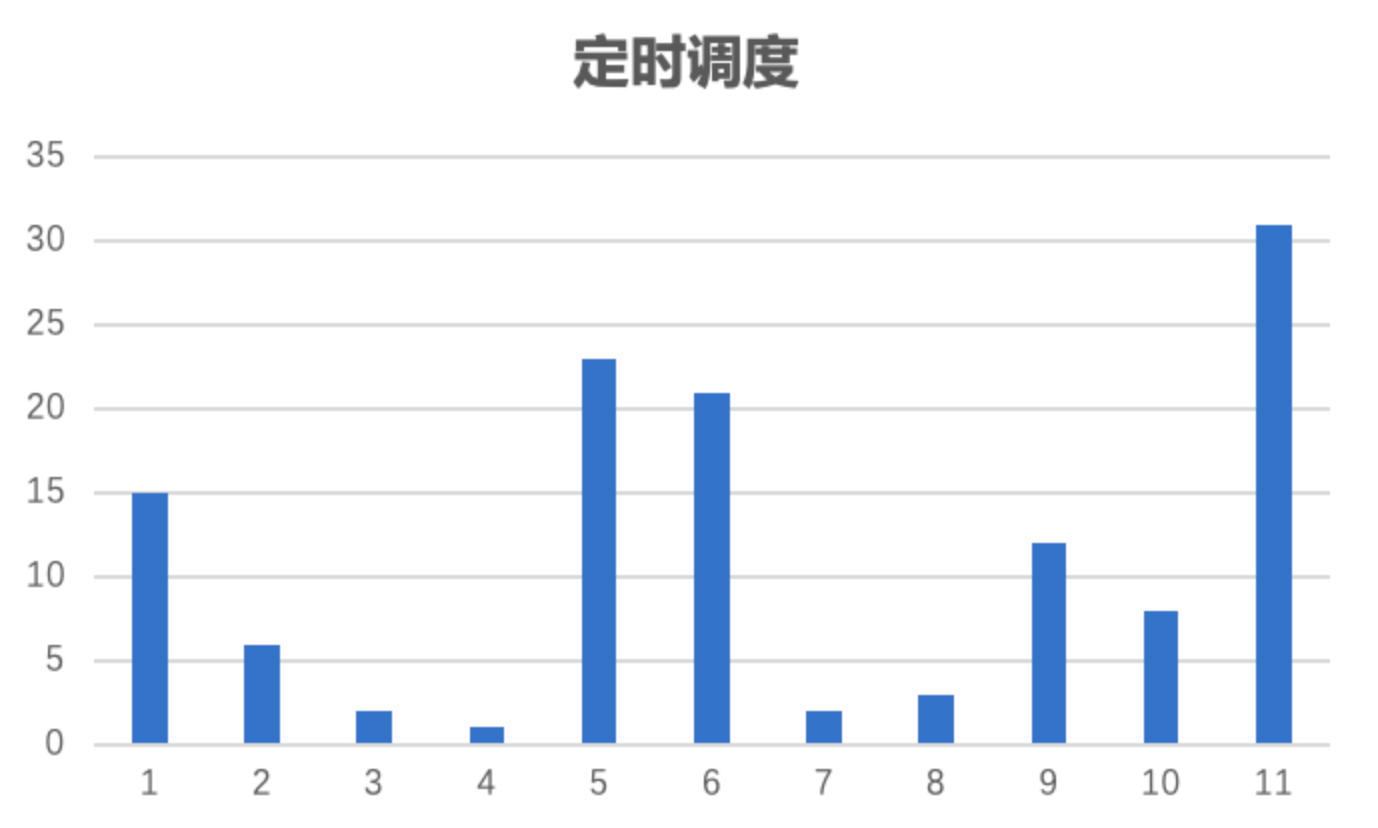
\includegraphics[width=1.0\textwidth]{小文件合并定时任务调度.png}
  \caption{定时任务调度合并文件数量}
  \label{fig:badge}
\end{figure}

如图3.7所示,两个任务分别合并了2个和7个小文件,而理想的状况是一个任务合并9个小文件,
该问题的核心点在于合并的任务无法知道当前的文件状态,因此需要一种计算规则来判断当前
一个区间内是否达到了发起合并任务的时刻,即需要计算出文件的状态,以作为合并任务调度的合并规则。

\begin{figure}[h]
  \centering
  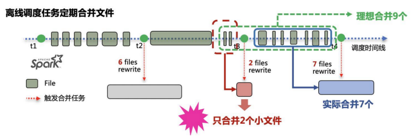
\includegraphics[width=1.0\textwidth]{小文件合并定时任务调度2.png}
  \caption{小文件合并理想示意图}
  \label{fig:badge}
\end{figure}

\section{系统非功能性需求}

(1)界面交互无障碍。系统应当提供给用户友好的交互界面,搭配各项可视化展示与适当的提示,提供给用户良好的服务使用体验;

(2)操作易用性。操作易用性要求软件开发时要减少不必要的操作步骤,方便用户的使用,采用高效的缓存机制,减少用户输入信息次数;

(3)系统安全性要求。系统安全性要求系统具备严格的权限访问控制机制,用户鉴权认证登录后,能够访问与之权限相对应的数据,只能使用其权限范围内的功能。另外要设置系统运行日志管理功能,及时发现运行过程中的问题;

(4)异常检测与系统可用性。由于要防止瞬时流量较高或者某个服务的波动引起的异常,系统需要有异常快速检测与上报功能,异常严重时还需要进行告警,保证系统整体可用;

(5)运行高效性。高效性是指系统在运行过程中的响应时间问题上,如登录时间、页面跳转时间、查询时间、页面刷新时间要短,非发起审核接口要在 1000ms 内相应,大规模数据地加载要在 2000ms 内完成;

(6)系统易维护性。在系统出现故障或者需要修改时要便于发现故障和判断需要修改部分所在位置,在修改时不会因局部的变动导致代码大篇算幅修改,最后是系统部署时间要短,将更多的时间用于开发;

(7)系统可移植性。可移植性要求系统对运行环境的适应性较强。所以在开发时要选用通用的程序设计语言,大部分系统都能够兼容的开发工具、数据库、插件;在界面设计时,要使用根据设备屏幕自适应的前端框架。

\section{本章小结}

在本章中首先对系统进行整体概述,明确项目目标以及应该具备的核心功能。
然后对数据源模块管理、元数据模块管理、数据入湖管理模块、数据探索模块、小文件合并功能五方面详细
描述系统的功能性需求。最后从系统性能需求、可用性、易用性等方面对系统的非功能性需求进行阐述。
